\section*{Lámina de caras paralelas}

\item En una lámina de caras paralelas indique la zona del espacio en que se observa interferencia para fuente puntual y para fuente extensa.
En el primer caso calcule la posición de las imágenes de la fuente. 


\item
\begin{minipage}[t][2.2cm]{0.6\textwidth}
En la lámina de caras paralelas que se indica en la figura, indique qué condición debe cumplirse para que los rayos 1 y 2 interfieran constructivamente.
Cuando eso sucede, ¿qué pasa con los rayos 3 y 4?
¿Qué sucede si se usan otras relaciones entre los índices? ($n_{1}>n_{2}>n_{3}$).
\end{minipage}
\begin{minipage}[c][1cm][t]{0.35\textwidth}
	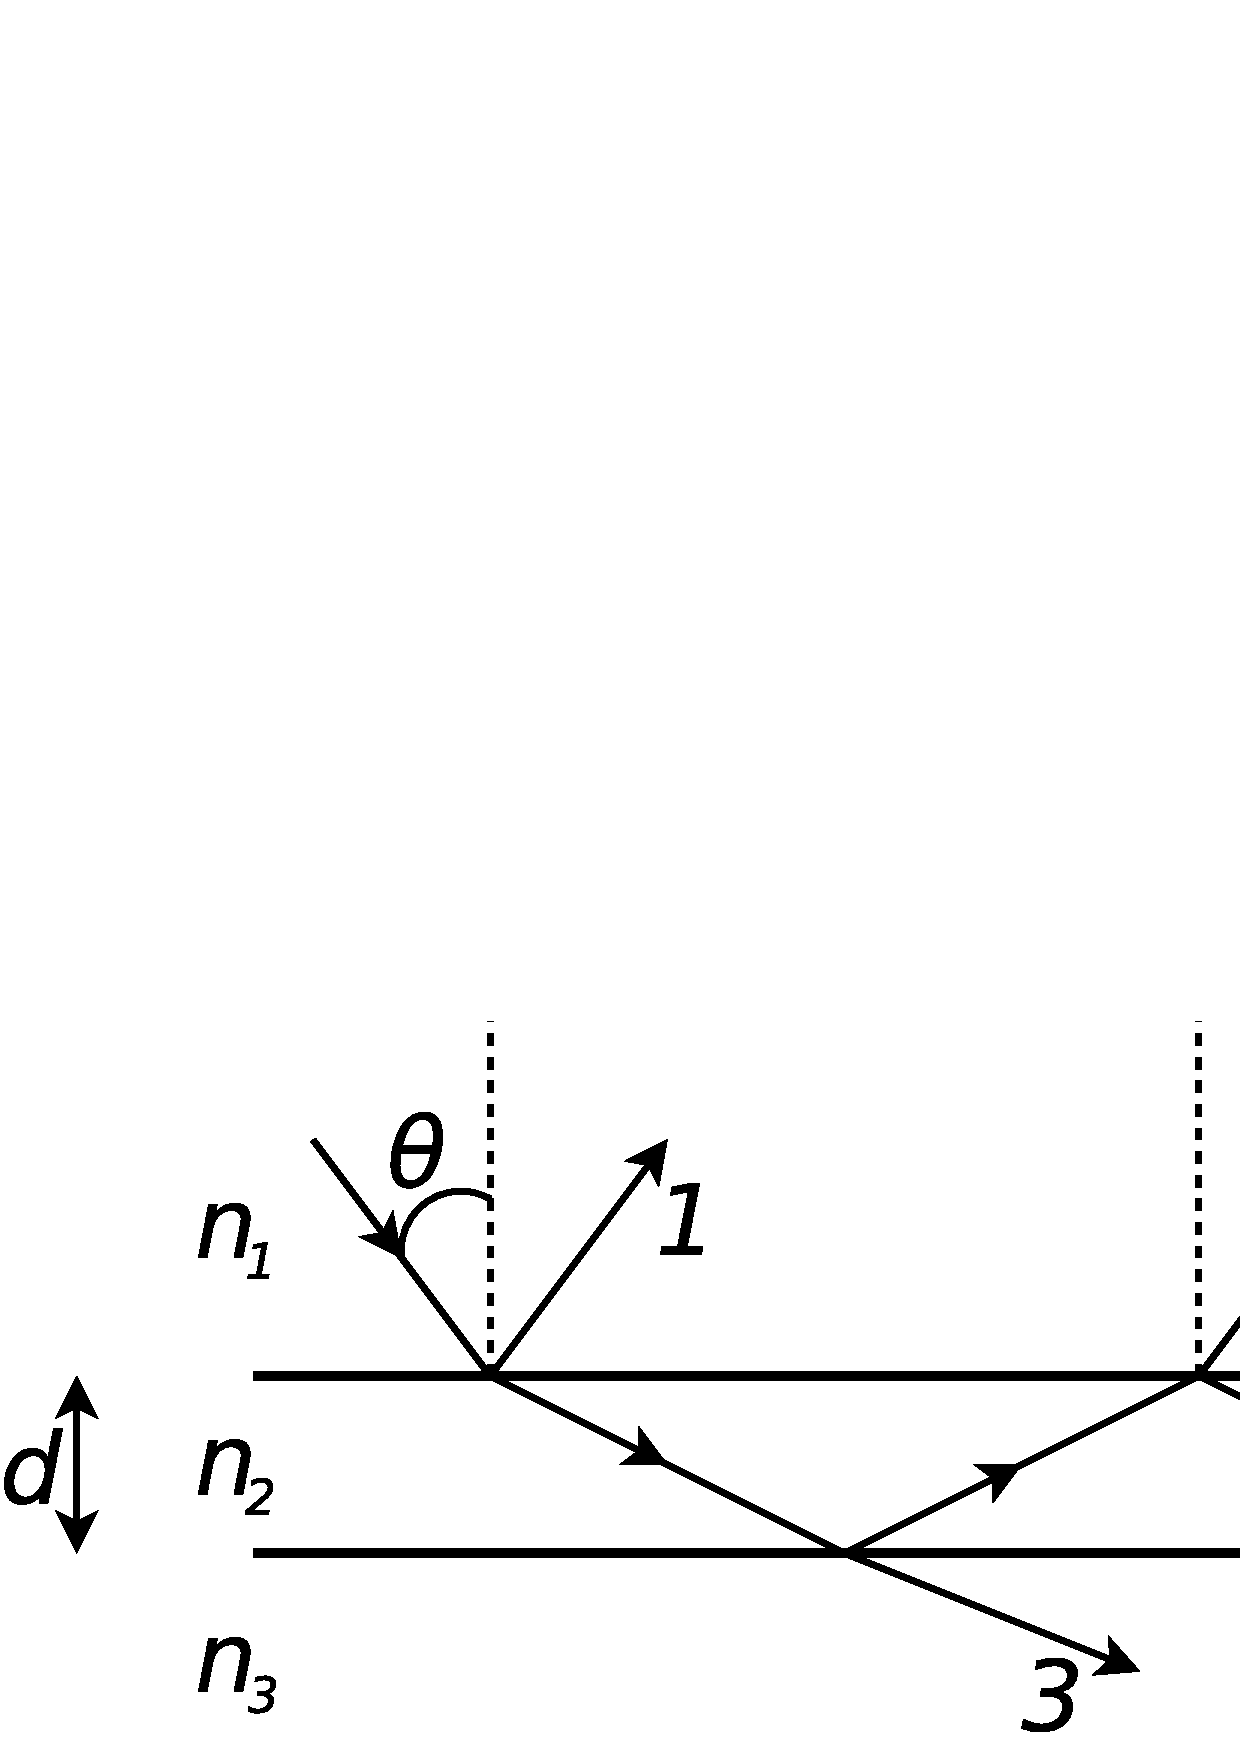
\includegraphics[width=\textwidth]{ej5-21}
\end{minipage}


\item Una lámina de vidrio de \SI{0.40}{\micro\metre} de espesor es iluminada por un haz de luz blanca normal a la lámina.
El índice de refracción es de \num{1.5}.
¿Qué longitudes de onda del espectro visible, \SIrange{400}{790}{\nano\metre}, serán intensificadas en el haz reflejado?



\item ¿Por qué se llaman franjas de igual inclinación a las que aparecen en una lámina de caras paralelas iluminada por una fuente extensa? 
